% *********************************************************************
% © 2021–2024 Jeremy Sylvestre
%
% Permission is granted to copy, distribute and/or modify this document
% under the terms of the GNU Free Documentation License, Version 1.3 or
% any later version published by the Free Software Foundation; with no
% Invariant Sections, no Front-Cover Texts, and no Back-Cover Texts. A
% copy of the license is included in the appendix entitled “GNU Free
% Documentation License” that appears in the output document of this
% PreTeXt source code. All trademarks™ are the registered® marks of
% their respective owners.
%
% *********************************************************************

\newcommand*{\xmin}{-2}
\newcommand*{\xmax}{2}
\newcommand*{\ymin}{-0.5}
\newcommand*{\ymax}{3}

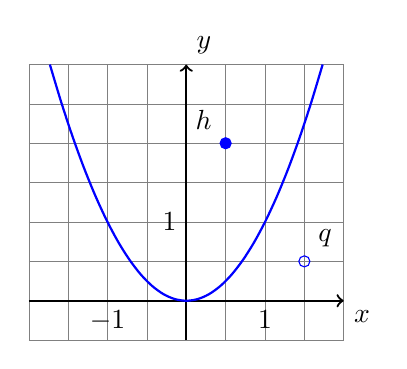
\begin{tikzpicture}
[
	closedpt/.style={circle,draw,fill,inner sep=0pt,minimum size=4pt},
	openpt/.style={circle,draw,inner sep=0pt,minimum size=4pt}
]

	% grid
	\foreach \x in {-2,-1.5,-1,...,2} {
		\draw[very thin,gray] (\x,\ymin) -- (\x,\ymax);
	}
	\foreach \y in {-0.5,0,0.5,...,3} {
		\draw[very thin,gray] (\xmin,\y) -- (\xmax,\y);
	}

	% label grid
	\foreach \x in {-1,1} {
		\node[below] at (\x,0) {$\x$};
	}
	\foreach \y in {1} {
		\node[left] at (0,1) {$\y$};
	}

	% example tick marks if not using grid
	% \draw (-1,0.1) -- (-1,-0.1) node[below] {$\scriptstyle -1$};
	% \draw (1,0.1) -- (1,-0.1) node[below] {$\scriptstyle 1$};
	% \draw (0.1,1) -- (-0.1,1) node[left] {$\scriptstyle 1$};

	% axes
	\draw[->,thick] (\xmin,0) -- (\xmax,0) node[below right] {$x$};
	\draw[->,thick] (0,\ymin) -- (0,\ymax) node[above right] {$y$};

	% example graph
	\draw[thick, blue, domain=-1.732:1.732,smooth] plot (\x,{\x * \x});

	% example points
	\node[blue,closedpt] at (0.5,2) (cl) [label=above left:$h$] {};
	\node[blue,openpt] at (1.5,0.5) (op) [label=above right:$q$] {};

\end{tikzpicture}
